\chapter{The Basis of Quantum Mechanics}

%**************** From Classical of Quantum Mechanics *************
%
\section{Introduction to Quantum Mechanics}

In this section we will give a brief introduction to some of the basic
properties of quantum mechanics. For a more thourough introduction to
quantum mechanics there are several references, among other
\cite{rohlf1994}, \cite{shankar1994} and \cite{hemmer1980}.

%*                    Wave-Particle Duality                    *
\subsection{Wave-Particle Duality}

Let us start out with a simple experiment. We send light through a
tiny\footnote{With 'tiny' we mean the approximate size of
the light's wave-length.} slit, and observe the
intensity-pattern on a screen behind the slit. The pattern is
illustrated in figure \ref{singleSlit}.

\begin{figure}[hbtp]
\begin{center}
  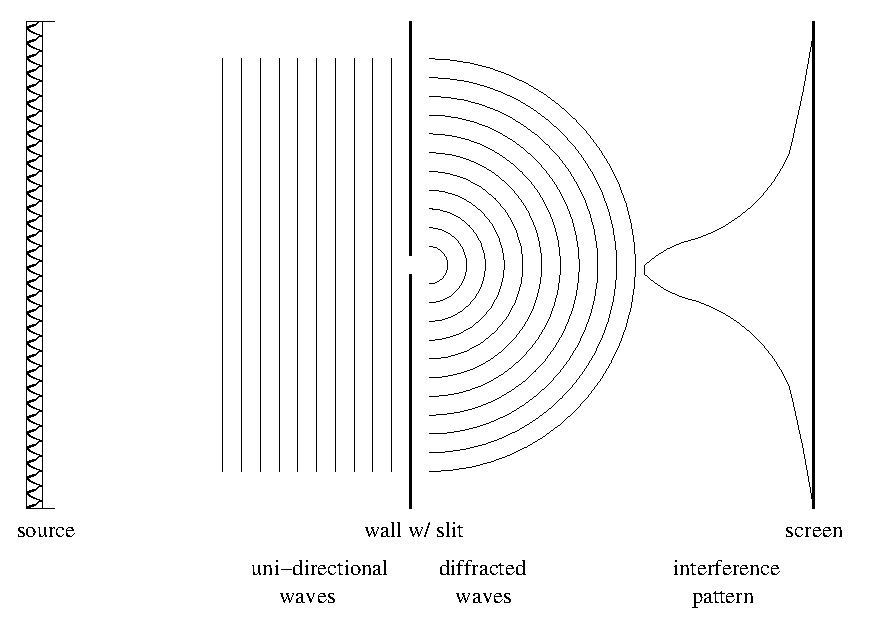
\epsfig{file=Basic_QM/singleSlit.eps, height=6cm}
  \caption{
    Single-slit diffraction
  }
  \label{singleSlit}
\end{center}
\end{figure}

We now expand the above experiment to include two slits, and get an
interference pattern as that given by figure \ref{doubleSlit}. 

\begin{figure}[hbtp]
\begin{center}
  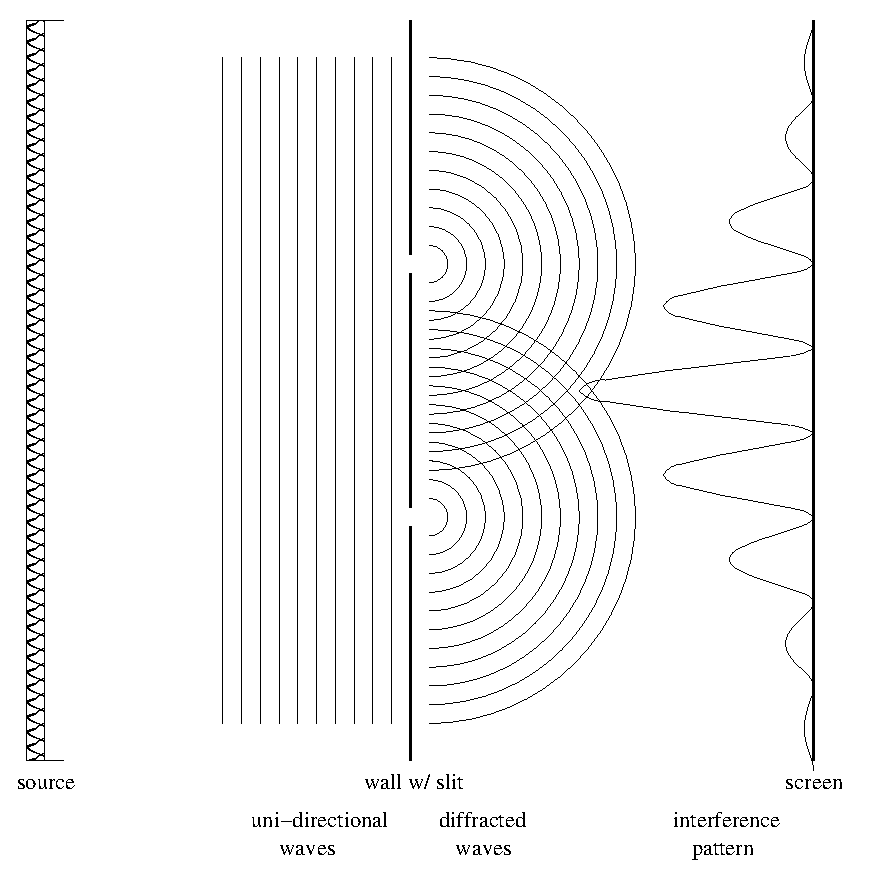
\epsfig{file=Basic_QM/doubleSlit.eps, height=9cm}
  \caption{
    Double-slit diffraction
  }
  \label{doubleSlit}
\end{center}
\end{figure}

If we sent classical particles through a double slit we would expect a
superposition of two single-slit intensity patterns. But this is not
what we actually observe for light.

In addition to the observed diffraction of light,
light may also be reflected and refracted. The reflection of light creates
the mirror image of a mountain on a still lake, and the light of
the sun refracted by a prism creates the rainbow hues. All the above
indicates that light has a wave-behavior. 
\newline
%
\newline

Lets us continue with yet another experiment. We direct light at a
conductive surface as illustrated in figure
\ref{photoElectricEffect}. 

\begin{figure}[hbtp]
\begin{center}
  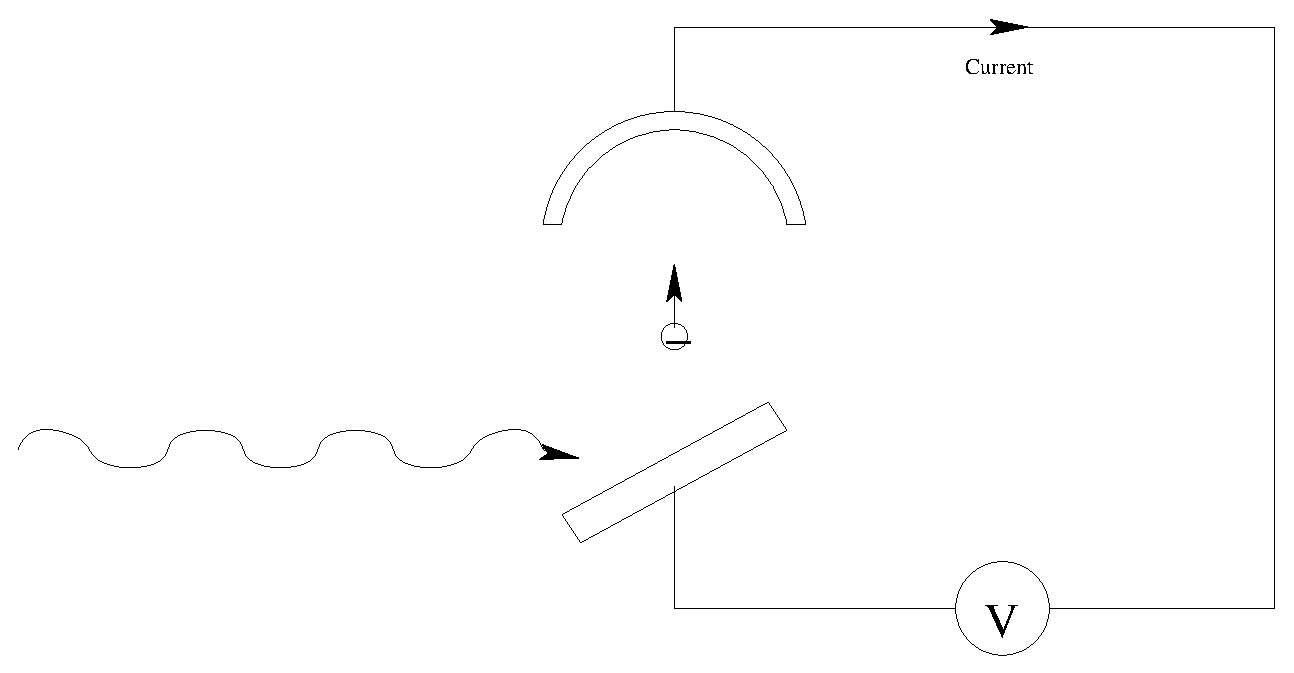
\epsfig{file=Basic_QM/photoElectricEffect.eps, height=6cm}
  \caption{
    Photo-electric effect
  }
  \label{photoElectricEffect}
\end{center}
\end{figure}


The light induces both a voltage and a current in the electric
circuit. What now if we increase the intensity of light? If light
were waves we would expect the voltage to increase, but only the
current is increased. This would indicate that light transfers only a
limited (even quantized!) amount of kinetic energy to the
electrons. But how can this be if light are waves? Who knows, but it's
in the nature of light. Furthermore, there is a lower limit of the
frequency needed to induce the photo-electric effect, dependent on the
photo-cathodic surface the light is directed at. Finally, if light
were waves, we would expect some time delay between when the light
source is turned on and the photo-electric effect is induced, but no
such delay is observed.

We have shown that light has both wave and particle
behavior, and this \emph{wave-particle duality} has no explanation in
classical physics. This duality is present in all objects, but is
measurable only for (sufficiently) small 'particles'.
\newline
%
\newline
%*                          DeBroglie Waves                       *
%\subsection{DeBroglie Waves}

In 1905 Einstein proposed that light has particle properties, 
and that each \emph{quanta} of light ({\bf photon}) has energy
  proportional to its frequency, $\nu$, 

\begin{equation*}
  E = h \nu
\end{equation*}

Here Planck's constant $h=6.626 \cdot 10^{-34} J \cdot s$, is a
fundamental constant of nature. Also in 1905, Einstein demonstrated, in
his special theory of relativity, that the photon has momentum like a
particle  

\begin{equation*}
  p = \frac{h} {\lambda}
\end{equation*}

This idea was generalized by Louis De Broglie, when he in 1924 proposed
that all matter have wave-like properties, and that they thus have a
wavelength ({\bf De Broglie wavelength}), 

\begin{equation*}
  \lambda = \frac{h} {p}
\end{equation*}



%*             Heisenberg's Uncertainty Principle             *
\subsection{Heisenberg's Uncertainty Principle}

In 1925 Heisenberg formulated his {\bf Uncertainty
  Principle}. Heisenberg's uncertainty principle states that one cannot
  measure a particle's position and momentum simultaneously with
  infinite precision.

\begin{equation*}
  \Delta x \Delta p \ge \frac{\hbar}{2}
\end{equation*}

Here $\Delta x$ and $\Delta p$ are the uncertainties in the position
and the momentum, respectively, and the \emph{reduced Plank's constant}
$\hbar = h/2\pi$. Also,

\begin{equation*}
  \Delta E \Delta t \ge \frac{\hbar}{2}
\end{equation*}

where $\Delta E$ and $\Delta t$ are the uncertainties energy and time,
respectively.

A consequence of the uncertainty principle is that
measuring the state of a microscopic system changes the system. 
\newline
%
\newline

Consider the double-slit experiment, depicted in figure
\ref{doubleSlit}, and reduce the intensity to allow only one
particle's to pass the slit at a time. What now? The interference
pattern in the figure now represents the particle's probability
distribution function. But how is this possible? In the classical way
of thinking the particle either passes the upper or the lower
slit. Following this line of thinking would lead to the superposition
of two single-slit experiments. This is not the case! So what then is
the solution? Either the photon is emitted from it's source at one
time, and then moves through both slits at the same time before
hitting the screen, or one simply cannot talk about a path at all.
Who knows?

So what then is the physicists approach?



%*                           The Quantum State                          *
\subsection{The Quantum State}

A proper description of a state allows all the known properties of
a system to be found. For a macroscopic system, the state of a
particle at a given time can be specified by a point in 
{\bf phase space}, i.e. the space spanned by the spatial coordinates
and the momentum coordinates. The energy, spin etc. of a particle, may 
all be found from the state of the particle.

In 1926 Erwin Schr\"odinger developed the idea of the \emph{complex}
{\bf wave function}, $\Psi = \Psi (\mathbf{x},t)$,
which is the state of microscopic systems. Unlike a trajectory the
wave-function has no independent reality. It only bears meaning in
conjunction with its complex conjugate $\Psi^*$ and an {\bf
  operator}. For example $\Psi^* \Psi = |\Psi|^2$ 
may be interpreted as a {\bf probability density} (here the operator
is the identity). For a given time
$t$ this has physical meaning when associated with a region in
space. Furthermore, this interpretation implies that the norm

\begin{equation*}
  \int\limits_{\Omega} |\Psi|^2 d\Omega = 1
\end{equation*}

where $\Omega$ is space. Thus, the wave-function must be
normalizable. 



%*                  Operators and Observables                          *
\subsection{Operators and Observables}

Every {\bf observable} (or measurable quantity) has an operator. The
information available in a wave-function is extracted by using the
operator to calculate an {\bf expectation value}. The expectation
value of an operator, $\left< \hat{{\cal O}} \right>$, is defined as

\begin{equation*}
  \left< \hat{{\cal O}} \right> 
  = \frac {\int \Psi^* \hat{{\cal O}} \Psi}  {\Psi^* \Psi}
\end{equation*}

For each classical variable
$\omega(\mathbf{x},\mathbf{p})$ there corresponds an operator $\Omega$
obtained by operator substitution of the two fundamental operators,

\begin{equation}
  \Omega(\mathbf{\hat{X}},\mathbf{\hat{P}}) = \omega(\mathbf{x} \to
  \mathbf{\hat{X}},\mathbf{p} \to \mathbf{\hat{P}})
  \label{operatorSubstitution}
\end{equation}

The fundamental operators of position and momentum are given by

\begin{equation*}
  \mathbf{\hat{X}} = \mathbf{x}
\end{equation*}

and

\begin{equation*}
  \mathbf{\hat{P}} = -i\hbar \nabla
\end{equation*}

respectively. 



%*            Commutators and Commuting Observables                   *
\subsection{Commutators and Commuting Observables}

An important feature in quantum mechanics is the 
{\bf commutator}. Given two operators $\hat{A}$ and $\hat{B}$ the
commutator is defined by

\begin{equation*}
  \left[ \hat{A}, \hat{B} \right] = \hat{A} \hat{B} - \hat{B} \hat{A}
\end{equation*}

A pair of operators are said to {\bf commute} if their commutator
equals zero. The values of the observables $A$ and $B$ can be known
both precisely and simultaneously, if and only if $\hat{A}$ and
$\hat{B}$ commute. The two fundamental position and momentum operators
does not commute:

\begin{equation*}
  \begin{split} 
  \left[ \hat{X_i}, \hat{P_i} \right] \Psi(\mathbf{x}, t) 
  &= \left[ x_i, -i \hbar \frac{\delta}{\delta x_i} \right] \Psi(\mathbf{x},t)
  = -i \hbar \left( x_i \frac{\delta}{\delta x_i} -
  \frac{\delta}{\delta x_i} x_i \right) \Psi(\mathbf{x},t) \\
  &= -i \hbar \left( x_i \frac{\delta}{\delta x_i} - \left[ x_i
  \frac{\delta}{\delta x_i} + 1 \right] \right) \Psi(\mathbf{x},t) 
  = i \hbar \Psi(\mathbf{x},t)
  \end{split}
\end{equation*}

i.e. $\left[ \hat{X_i}, \hat{P_i} \right] = i \hbar$. These two
observables may therefor not be known simultaneously, which is in
accordance with Heisenberg's uncertainty principle.


%*               Eigenfunctions and Eigenvalues                       *
\subsection{Eigenfunctions and Eigenvalues}

In the late nineteenth century, Anders \AA ngstom made wavelength
measurements of four visible lines emitted by hydrogen. This indicates
that the energy, and thereof the states, of the hydrogen atom are
quantized.  Quantum mechanical states can be described with 
{\bf eigenfunctions} of an operator. If a wave is in an
eigenstate, the observable has a corresponding 
{\bf eigenvalue}. The light waves of the hydrogen spectrum are
actually the photons emitted when the hydrogen atom goes from one
state to another. For an observable ${\cal O}$ with quantum operator
$\hat{{\cal O}}$ this yield the eigenvalue-problem,

\begin{equation*}
  \hat{{\cal O}} \Psi_n = {\cal O}_n \Psi_n
\end{equation*}

where $\Psi_n$ is an eigenstate and ${\cal O}_n$ is an eigenvalue.


%*                      The Hamiltonian                               *
\subsection{The Hamiltonian}

Classically, the total energy of a system is written in a systems 
{\bf Hamiltonian}, $H$. Usually, the Hamiltonian is defined as

\begin{equation*}
  H = T + V
\end{equation*}

where $T$ is the kinetic energy, and $V$ is the potential energy. The
kinetic energy operator of a one-particle system is

\begin{equation*}
  T = \frac{1}{2}m\mathbf{v}^2 = \frac{\mathbf{p}^2}{2m}
\end{equation*}

where $\mathbf{v}$ is the velocity and $\mathbf{p}$ is the
momentum. Performing operator substitution of the two fundamental
operators yield the quantum mechanical operator for the energy

\begin{equation*}
  \hat{H}(\mathbf{\hat{P}}, \mathbf{\hat{X}}, t) =
  \frac{\mathbf{\hat{P}}^2}{2m} + V(\mathbf{\hat{X}}, t)
\end{equation*}

Recalling that the fundamental operators of position and momentum are
given by 

\begin{equation*}
  \mathbf{\hat{X}} = \mathbf{x}
\end{equation*}

and

\begin{equation*}
  \mathbf{\hat{P}} = -i\hbar \nabla
\end{equation*}

the Hamiltonian of a one-particle quantum mechanical system reads

\begin{equation*}
  \hat{H}(\mathbf{x}, t) = -\frac{\hbar^2}{2m} \nabla^2 +
  V(\mathbf{x}, t)
\end{equation*}


%*                 The Schr\"odinger Equation                         *
\subsection{The Schr\"odinger Equation}

The Hamiltonian is the operator of the energy. And the
eigenvalue-problem posed by the Hamiltonian

\begin{equation*}
  \hat{H}(\mathbf{x}, t) \Psi_n(\mathbf{x}, t)  
  = E_n \Psi_n(\mathbf{x}, t) 
\end{equation*}

is called the stationary (or time-independent) Schr\"odinger
equation. The time-dependent Schr\"odinger equation

\begin{equation*}
  \hat{H}(\mathbf{x}, t) \Psi_n(\mathbf{x}, t)  
  = i\hbar \frac{\delta}{\delta t} \Psi_n(\mathbf{x}, t) 
\end{equation*}

will not be studied in this thesis. However, as a fundamental equation
of quantum mechanics it sort of found its way into this thesis anyhow.

%*                     The Hilbert Space                              *
\subsection{The Hilbert Space}

A common formulation of quantum mechanics is by means of linear
algebra. In this formulation every state is represented as a (usually
infinite dimensional) complex vector, and an operator is represented
as a complex, linear and hermitian matrix. 
The {\bf Hilbert space} is the (usually infinite dimensional) complex
linear state space. The Hilbert space is dual in that every vector
$\Psi$ is associated with the dual vector $\Psi^*$.



%*************** The Postulates of Quantum Mechanics **************
%*
%*
\subsection{The Postulates of Quantum Mechanics}

We are now ready to formulate the postulates of quantum mechanics. The
postulates fall naturally into two sets: the first three, which tell
us how the system is depicted at a given time, and the last, which
specifies how this picture changes with time. 
\newline

%*                     The First Postulate                              *
%\subsection{The First Postulate}

{\bf \large Postulate 1}
\emph{
The state of a quantum mechanical particle is described by a vector
$\Psi$ in a Hilbert space ${\cal H}$. All the possible states of the
particle are ${\cal H}$ except the zero vector.
\newline
}

The first postulate states that a particle is described as a vector in
the Hilbert space. So a classical particle with finite\footnote{Six
  degrees of freedom for the three-dimensional case.} degrees of
freedom, $\mathbf{x}$ and $\mathbf{p}$, in classical
mechanics, now has infinite degrees of freedom. 
\newline

%*                     The Second Postulate                              *
%\subsection{The Second Postulate}

The second postulate defines the quantum operator for the observables
(or measurable quantities). !!! Some more intro here !!!
\newline

{\bf \large Postulate 2}
\emph{
Every observable are represented by an Hermitian linear operator in
${\cal H}$. For every classical dynamical variable
$\omega(\mathbf{x},\mathbf{p})$ there corresponds an operator $\Omega$ 
obtained by operator substitution of the fundamental position and
momentum operators $\mathbf{X}$ and $\mathbf{P}$, respectively:
}
%
\begin{equation*}
  \Omega(\mathbf{X},\mathbf{P}) = \omega(\mathbf{x} \to
  \mathbf{X},\mathbf{p} \to \mathbf{P})
\end{equation*}
%
\emph{
The components of $\mathbf{X}$ and $\mathbf{P}$ are operators defined
through the fundamental commutation relation
}

\begin{equation*}
  \left[ X_i, P_j \right] = i \hbar \delta_{ij}
\end{equation*}

%*                     The Third Postulate                              *
%\subsection{The Third Postulate}

{\bf \large Postulate 3}
\emph{
The only possible values obtainable in an (ideal) measurement of an
observable $\Omega$ are its eigenvalues $\omega_n$. Each have a
probability
}
%
\begin{equation*}
  P(\omega_n) = \frac{\int \Psi^* \Phi_n }{\int \Psi^* \Psi }
\end{equation*}
%
\emph{
with $\Phi_n$ the eigenfunction corresponding to the eigenvalue
$\omega_n$. Immediately after a measurement the state collapses into
$\Phi_n$.
}
\newline

Note that the eigenvalues may have a continuous spectrum.
\newline


%*                     The Fourth Postulate                              *
%\subsection{The Fourth Postulate}

The fourth and final postulate defines the Schr\"odinger equation.
\newline

{\bf \large Postulate 4}
\emph{
The time development of the quantum state $\Psi$ is given by the time
dependent Schr\"odinger equation,
}

\begin{equation*}
  \hat{H} \Psi(\mathbf{x},t) = i\hbar \frac{\delta}{\delta
  t}\Psi(\mathbf{x},t) 
\end{equation*}

%*                Bosons and Fermions                                *
\subsection{Bosons and Fermions}

spin half or integer


%*                       The Pauli Principle                         *
\subsection{The Pauli Principle}



